\documentclass[1p]{elsarticle_modified}
%\bibliographystyle{elsarticle-num}

%\usepackage[colorlinks]{hyperref}
%\usepackage{abbrmath_seonhwa} %\Abb, \Ascr, \Acal ,\Abf, \Afrak
\usepackage{amsfonts}
\usepackage{amssymb}
\usepackage{amsmath}
\usepackage{amsthm}
\usepackage{scalefnt}
\usepackage{amsbsy}
\usepackage{kotex}
\usepackage{caption}
\usepackage{subfig}
\usepackage{color}
\usepackage{graphicx}
\usepackage{xcolor} %% white, black, red, green, blue, cyan, magenta, yellow
\usepackage{float}
\usepackage{setspace}
\usepackage{hyperref}

\usepackage{tikz}
\usetikzlibrary{arrows}

\usepackage{multirow}
\usepackage{array} % fixed length table
\usepackage{hhline}

%%%%%%%%%%%%%%%%%%%%%
\makeatletter
\renewcommand*\env@matrix[1][\arraystretch]{%
	\edef\arraystretch{#1}%
	\hskip -\arraycolsep
	\let\@ifnextchar\new@ifnextchar
	\array{*\c@MaxMatrixCols c}}
\makeatother %https://tex.stackexchange.com/questions/14071/how-can-i-increase-the-line-spacing-in-a-matrix
%%%%%%%%%%%%%%%

\usepackage[normalem]{ulem}

\newcommand{\msout}[1]{\ifmmode\text{\sout{\ensuremath{#1}}}\else\sout{#1}\fi}
%SOURCE: \msout is \stkout macro in https://tex.stackexchange.com/questions/20609/strikeout-in-math-mode

\newcommand{\cancel}[1]{
	\ifmmode
	{\color{red}\msout{#1}}
	\else
	{\color{red}\sout{#1}}
	\fi
}

\newcommand{\add}[1]{
	{\color{blue}\uwave{#1}}
}

\newcommand{\replace}[2]{
	\ifmmode
	{\color{red}\msout{#1}}{\color{blue}\uwave{#2}}
	\else
	{\color{red}\sout{#1}}{\color{blue}\uwave{#2}}
	\fi
}

\newcommand{\Sol}{\mathcal{S}} %segment
\newcommand{\D}{D} %diagram
\newcommand{\A}{\mathcal{A}} %arc


%%%%%%%%%%%%%%%%%%%%%%%%%%%%%5 test

\def\sl{\operatorname{\textup{SL}}(2,\Cbb)}
\def\psl{\operatorname{\textup{PSL}}(2,\Cbb)}
\def\quan{\mkern 1mu \triangleright \mkern 1mu}

\theoremstyle{definition}
\newtheorem{thm}{Theorem}[section]
\newtheorem{prop}[thm]{Proposition}
\newtheorem{lem}[thm]{Lemma}
\newtheorem{ques}[thm]{Question}
\newtheorem{cor}[thm]{Corollary}
\newtheorem{defn}[thm]{Definition}
\newtheorem{exam}[thm]{Example}
\newtheorem{rmk}[thm]{Remark}
\newtheorem{alg}[thm]{Algorithm}

\newcommand{\I}{\sqrt{-1}}
\begin{document}

%\begin{frontmatter}
%
%\title{Boundary parabolic representations of knots up to 8 crossings}
%
%%% Group authors per affiliation:
%\author{Yunhi Cho} 
%\address{Department of Mathematics, University of Seoul, Seoul, Korea}
%\ead{yhcho@uos.ac.kr}
%
%
%\author{Seonhwa Kim} %\fnref{s_kim}}
%\address{Center for Geometry and Physics, Institute for Basic Science, Pohang, 37673, Korea}
%\ead{ryeona17@ibs.re.kr}
%
%\author{Hyuk Kim}
%\address{Department of Mathematical Sciences, Seoul National University, Seoul 08826, Korea}
%\ead{hyukkim@snu.ac.kr}
%
%\author{Seokbeom Yoon}
%\address{Department of Mathematical Sciences, Seoul National University, Seoul, 08826,  Korea}
%\ead{sbyoon15@snu.ac.kr}
%
%\begin{abstract}
%We find all boundary parabolic representation of knots up to 8 crossings.
%
%\end{abstract}
%\begin{keyword}
%    \MSC[2010] 57M25 
%\end{keyword}
%
%\end{frontmatter}

%\linenumbers
%\tableofcontents
%
\newcommand\colored[1]{\textcolor{white}{\rule[-0.35ex]{0.8em}{1.4ex}}\kern-0.8em\color{red} #1}%
%\newcommand\colored[1]{\textcolor{white}{ #1}\kern-2.17ex	\textcolor{white}{ #1}\kern-1.81ex	\textcolor{white}{ #1}\kern-2.15ex\color{red}#1	}

{\Large $\underline{10_{161}~(K10n_{31})}$}

\setlength{\tabcolsep}{10pt}
\renewcommand{\arraystretch}{1.6}
\vspace{1cm}\begin{tabular}{m{100pt}>{\centering\arraybackslash}m{274pt}}
\multirow{5}{120pt}{
	\centering
	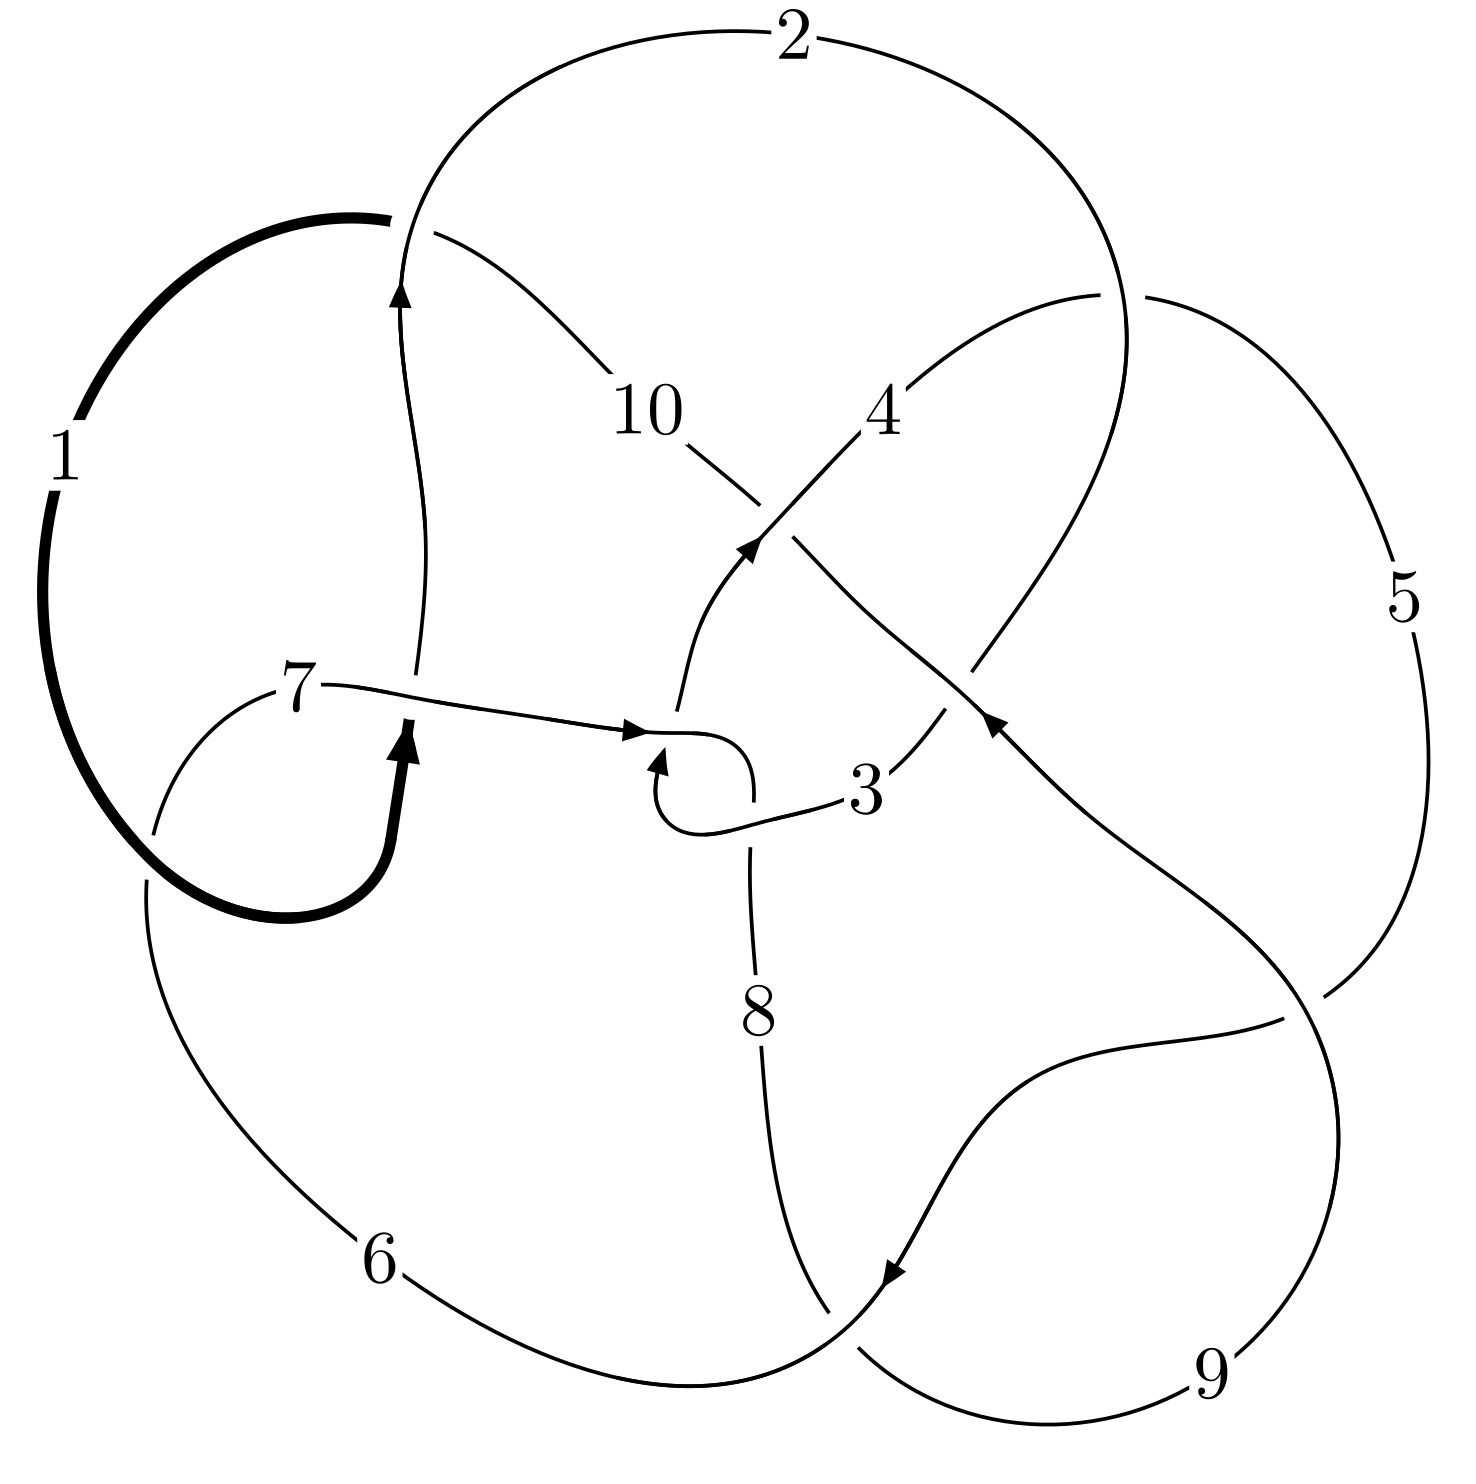
\includegraphics[width=112pt]{../../../GIT/diagram.site/Diagrams/png/245_10_161.png}\\
\ \ \ A knot diagram\footnotemark}&
\allowdisplaybreaks
\textbf{Linearized knot diagam} \\
\cline{2-2}
 &
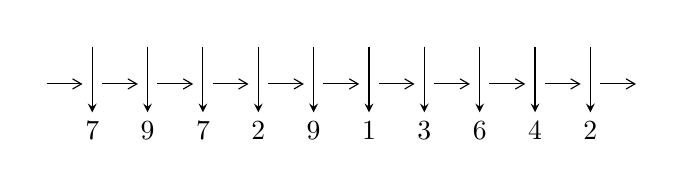
\begin{tikzpicture}[x=20pt, y=17pt]
	% nodes
	\node (C0) at (0, 0) {};
	\node (C1) at (1, 0) {};
	\node (C1U) at (1, +1) {};
	\node (C1D) at (1, -1) {7};

	\node (C2) at (2, 0) {};
	\node (C2U) at (2, +1) {};
	\node (C2D) at (2, -1) {9};

	\node (C3) at (3, 0) {};
	\node (C3U) at (3, +1) {};
	\node (C3D) at (3, -1) {7};

	\node (C4) at (4, 0) {};
	\node (C4U) at (4, +1) {};
	\node (C4D) at (4, -1) {2};

	\node (C5) at (5, 0) {};
	\node (C5U) at (5, +1) {};
	\node (C5D) at (5, -1) {9};

	\node (C6) at (6, 0) {};
	\node (C6U) at (6, +1) {};
	\node (C6D) at (6, -1) {1};

	\node (C7) at (7, 0) {};
	\node (C7U) at (7, +1) {};
	\node (C7D) at (7, -1) {3};

	\node (C8) at (8, 0) {};
	\node (C8U) at (8, +1) {};
	\node (C8D) at (8, -1) {6};

	\node (C9) at (9, 0) {};
	\node (C9U) at (9, +1) {};
	\node (C9D) at (9, -1) {4};

	\node (C10) at (10, 0) {};
	\node (C10U) at (10, +1) {};
	\node (C10D) at (10, -1) {2};
	\node (C11) at (11, 0) {};

	% arrows
	\draw[->,>={angle 60}]
	(C0) edge (C1) (C1) edge (C2) (C2) edge (C3) (C3) edge (C4) (C4) edge (C5) (C5) edge (C6) (C6) edge (C7) (C7) edge (C8) (C8) edge (C9) (C9) edge (C10) (C10) edge (C11) ;	\draw[->,>=stealth]
	(C1U) edge (C1D) (C2U) edge (C2D) (C3U) edge (C3D) (C4U) edge (C4D) (C5U) edge (C5D) (C6U) edge (C6D) (C7U) edge (C7D) (C8U) edge (C8D) (C9U) edge (C9D) (C10U) edge (C10D) ;
	\end{tikzpicture} \\
\hhline{~~} \\& 
\textbf{Solving Sequence} \\ \cline{2-2} 
 &
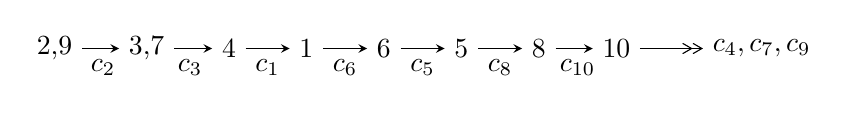
\begin{tikzpicture}[x=28pt, y=7pt]
	% node
	\node (A0) at (-1/8, 0) {2,9};
	\node (A1) at (17/16, 0) {3,7};
	\node (A2) at (17/8, 0) {4};
	\node (A3) at (25/8, 0) {1};
	\node (A4) at (33/8, 0) {6};
	\node (A5) at (41/8, 0) {5};
	\node (A6) at (49/8, 0) {8};
	\node (A7) at (57/8, 0) {10};
	\node (C1) at (1/2, -1) {$c_{2}$};
	\node (C2) at (13/8, -1) {$c_{3}$};
	\node (C3) at (21/8, -1) {$c_{1}$};
	\node (C4) at (29/8, -1) {$c_{6}$};
	\node (C5) at (37/8, -1) {$c_{5}$};
	\node (C6) at (45/8, -1) {$c_{8}$};
	\node (C7) at (53/8, -1) {$c_{10}$};
	\node (A8) at (9, 0) {$c_{4},c_{7},c_{9}$};

	% edge
	\draw[->,>=stealth]	
	(A0) edge (A1) (A1) edge (A2) (A2) edge (A3) (A3) edge (A4) (A4) edge (A5) (A5) edge (A6) (A6) edge (A7) ;
	\draw[->>,>={angle 60}]	
	(A7) edge (A8);
\end{tikzpicture} \\ 

\end{tabular} \\

\footnotetext{
The image of knot diagram is generated by the software ``\textbf{Draw programme}" developed by Andrew Bartholomew(\url{http://www.layer8.co.uk/maths/draw/index.htm\#Running-draw}), where we modified some parts for our purpose(\url{https://github.com/CATsTAILs/LinksPainter}).
}\phantom \\ \newline 
\centering \textbf{Ideals for irreducible components\footnotemark of $X_{\text{par}}$} 
 
\begin{align*}
I^u_{1}&=\langle 
-29 u^5+62 u^4-233 u^3-17 u^2+73 b-178 u-27,\;-15 u^5+22 u^4-118 u^3-39 u^2+73 a-228 u-19,\\
\phantom{I^u_{1}}&\phantom{= \langle  }u^6-2 u^5+8 u^4+u^3+7 u^2- u-1\rangle \\
I^u_{2}&=\langle 
u^2+b+u,\;u^3+u^2+a- u,\;u^4+u^3-1\rangle \\
\\
\end{align*}
\raggedright * 2 irreducible components of $\dim_{\mathbb{C}}=0$, with total 10 representations.\\
\footnotetext{All coefficients of polynomials are rational numbers. But the coefficients are sometimes approximated in decimal forms when there is not enough margin.}
\newpage
\renewcommand{\arraystretch}{1}
\centering \section*{I. $I^u_{1}= \langle -29 u^5+62 u^4+\cdots+73 b-27,\;-15 u^5+22 u^4+\cdots+73 a-19,\;u^6-2 u^5+8 u^4+u^3+7 u^2- u-1 \rangle$}
\flushleft \textbf{(i) Arc colorings}\\
\begin{tabular}{m{7pt} m{180pt} m{7pt} m{180pt} }
\flushright $a_{2}=$&$\begin{pmatrix}1\\0\end{pmatrix}$ \\
\flushright $a_{9}=$&$\begin{pmatrix}0\\u\end{pmatrix}$ \\
\flushright $a_{3}=$&$\begin{pmatrix}1\\u^2\end{pmatrix}$ \\
\flushright $a_{7}=$&$\begin{pmatrix}0.205479 u^{5}-0.301370 u^{4}+\cdots+3.12329 u+0.260274\\0.397260 u^{5}-0.849315 u^{4}+\cdots+2.43836 u+0.369863\end{pmatrix}$ \\
\flushright $a_{4}=$&$\begin{pmatrix}0.260274 u^{5}-0.315068 u^{4}+\cdots+2.35616 u+1.86301\\0.260274 u^{5}-0.315068 u^{4}+\cdots+2.35616 u+0.863014\end{pmatrix}$ \\
\flushright $a_{1}=$&$\begin{pmatrix}-0.205479 u^{5}+0.301370 u^{4}+\cdots-3.12329 u-0.260274\\-0.452055 u^{5}+0.863014 u^{4}+\cdots-2.67123 u-0.972603\end{pmatrix}$ \\
\flushright $a_{6}=$&$\begin{pmatrix}-1\\-0.260274 u^{5}+0.315068 u^{4}+\cdots-2.35616 u-0.863014\end{pmatrix}$ \\
\flushright $a_{5}=$&$\begin{pmatrix}-1\\-0.260274 u^{5}+0.315068 u^{4}+\cdots-2.35616 u-0.863014\end{pmatrix}$ \\
\flushright $a_{8}=$&$\begin{pmatrix}u\\0.205479 u^{5}-0.301370 u^{4}+\cdots+2.12329 u+0.260274\end{pmatrix}$ \\
\flushright $a_{10}=$&$\begin{pmatrix}-0.657534 u^{5}+1.16438 u^{4}+\cdots-5.79452 u-1.23288\\-0.452055 u^{5}+0.863014 u^{4}+\cdots-2.67123 u-0.972603\end{pmatrix}$\\&\end{tabular}
\flushleft \textbf{(ii) Obstruction class $= -1$}\\~\\
\flushleft \textbf{(iii) Cusp Shapes $= \frac{145}{73} u^5-\frac{310}{73} u^4+\frac{1165}{73} u^3+\frac{85}{73} u^2+\frac{744}{73} u-\frac{887}{73}$}\\~\\
\newpage\renewcommand{\arraystretch}{1}
\flushleft \textbf{(iv) u-Polynomials at the component}\newline \\
\begin{tabular}{m{50pt}|m{274pt}}
Crossings & \hspace{64pt}u-Polynomials at each crossing \\
\hline $$\begin{aligned}c_{1},c_{6}\end{aligned}$$&$\begin{aligned}
&u^6-6 u^5+16 u^4-21 u^3+11 u^2+2 u-4
\end{aligned}$\\
\hline $$\begin{aligned}c_{2},c_{5},c_{8}\end{aligned}$$&$\begin{aligned}
&u^6-2 u^5+8 u^4+u^3+7 u^2- u-1
\end{aligned}$\\
\hline $$\begin{aligned}c_{3},c_{7},c_{9}\end{aligned}$$&$\begin{aligned}
&u^6+u^5+9 u^4-11 u^3-4 u^2-2 u-1
\end{aligned}$\\
\hline $$\begin{aligned}c_{4}\end{aligned}$$&$\begin{aligned}
&u^6-3 u^5-3 u^4+15 u^3-10 u^2+1
\end{aligned}$\\
\hline $$\begin{aligned}c_{10}\end{aligned}$$&$\begin{aligned}
&u^6+4 u^5+26 u^4+73 u^3+77 u^2+92 u+16
\end{aligned}$\\
\hline
\end{tabular}\\~\\
\newpage\renewcommand{\arraystretch}{1}
\flushleft \textbf{(v) Riley Polynomials at the component}\newline \\
\begin{tabular}{m{50pt}|m{274pt}}
Crossings & \hspace{64pt}Riley Polynomials at each crossing \\
\hline $$\begin{aligned}c_{1},c_{6}\end{aligned}$$&$\begin{aligned}
&y^6-4 y^5+26 y^4-73 y^3+77 y^2-92 y+16
\end{aligned}$\\
\hline $$\begin{aligned}c_{2},c_{5},c_{8}\end{aligned}$$&$\begin{aligned}
&y^6+12 y^5+82 y^4+105 y^3+35 y^2-15 y+1
\end{aligned}$\\
\hline $$\begin{aligned}c_{3},c_{7},c_{9}\end{aligned}$$&$\begin{aligned}
&y^6+17 y^5+95 y^4-191 y^3-46 y^2+4 y+1
\end{aligned}$\\
\hline $$\begin{aligned}c_{4}\end{aligned}$$&$\begin{aligned}
&y^6-15 y^5+79 y^4-163 y^3+94 y^2-20 y+1
\end{aligned}$\\
\hline $$\begin{aligned}c_{10}\end{aligned}$$&$\begin{aligned}
&y^6+36 y^5+246 y^4-2029 y^3-6671 y^2-6000 y+256
\end{aligned}$\\
\hline
\end{tabular}\\~\\
\newpage\flushleft \textbf{(vi) Complex Volumes and Cusp Shapes}
$$\begin{array}{c|c|c}  
\text{Solutions to }I^u_{1}& \I (\text{vol} + \sqrt{-1}CS) & \text{Cusp shape}\\
 \hline 
\begin{aligned}
u &= -0.244201 + 0.971888 I \\
a &= -0.24405 + 1.39509 I \\
b &= \phantom{-}0.878332 - 0.695514 I\end{aligned}
 & \phantom{-}2.08576 + 2.67800 I & -9.11994 - 5.42135 I \\ \hline\begin{aligned}
u &= -0.244201 - 0.971888 I \\
a &= -0.24405 - 1.39509 I \\
b &= \phantom{-}0.878332 + 0.695514 I\end{aligned}
 & \phantom{-}2.08576 - 2.67800 I & -9.11994 + 5.42135 I \\ \hline\begin{aligned}
u &= \phantom{-}0.403945\phantom{ +0.000000I} \\
a &= \phantom{-}1.70981\phantom{ +0.000000I} \\
b &= \phantom{-}1.58486\phantom{ +0.000000I}\end{aligned}
 & -7.78420\phantom{ +0.000000I} & -6.88360\phantom{ +0.000000I} \\ \hline\begin{aligned}
u &= -0.304480\phantom{ +0.000000I} \\
a &= -0.689933\phantom{ +0.000000I} \\
b &= -0.449415\phantom{ +0.000000I}\end{aligned}
 & -0.637429\phantom{ +0.000000I} & -15.6380\phantom{ +0.000000I} \\ \hline\begin{aligned}
u &= \phantom{-}1.19447 + 2.58259 I \\
a &= \phantom{-}0.234107 - 0.606474 I \\
b &= \phantom{-}1.55395 + 1.43504 I\end{aligned}
 & \phantom{-}13.6396 - 5.6388 I & -8.61921 + 2.01004 I \\ \hline\begin{aligned}
u &= \phantom{-}1.19447 - 2.58259 I \\
a &= \phantom{-}0.234107 + 0.606474 I \\
b &= \phantom{-}1.55395 - 1.43504 I\end{aligned}
 & \phantom{-}13.6396 + 5.6388 I & -8.61921 - 2.01004 I\\
 \hline 
 \end{array}$$\newpage\newpage\renewcommand{\arraystretch}{1}
\centering \section*{II. $I^u_{2}= \langle u^2+b+u,\;u^3+u^2+a- u,\;u^4+u^3-1 \rangle$}
\flushleft \textbf{(i) Arc colorings}\\
\begin{tabular}{m{7pt} m{180pt} m{7pt} m{180pt} }
\flushright $a_{2}=$&$\begin{pmatrix}1\\0\end{pmatrix}$ \\
\flushright $a_{9}=$&$\begin{pmatrix}0\\u\end{pmatrix}$ \\
\flushright $a_{3}=$&$\begin{pmatrix}1\\u^2\end{pmatrix}$ \\
\flushright $a_{7}=$&$\begin{pmatrix}- u^3- u^2+u\\- u^2- u\end{pmatrix}$ \\
\flushright $a_{4}=$&$\begin{pmatrix}u^2+u\\u^2+u+1\end{pmatrix}$ \\
\flushright $a_{1}=$&$\begin{pmatrix}u^3+u^2- u\\- u^3- u^2-1\end{pmatrix}$ \\
\flushright $a_{6}=$&$\begin{pmatrix}-1\\u+1\end{pmatrix}$ \\
\flushright $a_{5}=$&$\begin{pmatrix}-1\\u^2+u+1\end{pmatrix}$ \\
\flushright $a_{8}=$&$\begin{pmatrix}u\\- u^2\end{pmatrix}$ \\
\flushright $a_{10}=$&$\begin{pmatrix}- u-1\\- u^3- u^2-1\end{pmatrix}$\\&\end{tabular}
\flushleft \textbf{(ii) Obstruction class $= 1$}\\~\\
\flushleft \textbf{(iii) Cusp Shapes $= -2 u^3-7 u^2-7 u-10$}\\~\\
\newpage\renewcommand{\arraystretch}{1}
\flushleft \textbf{(iv) u-Polynomials at the component}\newline \\
\begin{tabular}{m{50pt}|m{274pt}}
Crossings & \hspace{64pt}u-Polynomials at each crossing \\
\hline $$\begin{aligned}c_{1}\end{aligned}$$&$\begin{aligned}
&u^4-2 u^2+u+1
\end{aligned}$\\
\hline $$\begin{aligned}c_{2},c_{8}\end{aligned}$$&$\begin{aligned}
&u^4+u^3-1
\end{aligned}$\\
\hline $$\begin{aligned}c_{3},c_{9}\end{aligned}$$&$\begin{aligned}
&u^4+u-1
\end{aligned}$\\
\hline $$\begin{aligned}c_{4}\end{aligned}$$&$\begin{aligned}
&u^4+4 u^3+4 u^2+u+1
\end{aligned}$\\
\hline $$\begin{aligned}c_{5}\end{aligned}$$&$\begin{aligned}
&u^4- u^3-1
\end{aligned}$\\
\hline $$\begin{aligned}c_{6}\end{aligned}$$&$\begin{aligned}
&u^4-2 u^2- u+1
\end{aligned}$\\
\hline $$\begin{aligned}c_{7}\end{aligned}$$&$\begin{aligned}
&u^4- u-1
\end{aligned}$\\
\hline $$\begin{aligned}c_{10}\end{aligned}$$&$\begin{aligned}
&u^4-4 u^3+6 u^2-5 u+1
\end{aligned}$\\
\hline
\end{tabular}\\~\\
\newpage\renewcommand{\arraystretch}{1}
\flushleft \textbf{(v) Riley Polynomials at the component}\newline \\
\begin{tabular}{m{50pt}|m{274pt}}
Crossings & \hspace{64pt}Riley Polynomials at each crossing \\
\hline $$\begin{aligned}c_{1},c_{6}\end{aligned}$$&$\begin{aligned}
&y^4-4 y^3+6 y^2-5 y+1
\end{aligned}$\\
\hline $$\begin{aligned}c_{2},c_{5},c_{8}\end{aligned}$$&$\begin{aligned}
&y^4- y^3-2 y^2+1
\end{aligned}$\\
\hline $$\begin{aligned}c_{3},c_{7},c_{9}\end{aligned}$$&$\begin{aligned}
&y^4-2 y^2- y+1
\end{aligned}$\\
\hline $$\begin{aligned}c_{4}\end{aligned}$$&$\begin{aligned}
&y^4-8 y^3+10 y^2+7 y+1
\end{aligned}$\\
\hline $$\begin{aligned}c_{10}\end{aligned}$$&$\begin{aligned}
&y^4-4 y^3-2 y^2-13 y+1
\end{aligned}$\\
\hline
\end{tabular}\\~\\
\newpage\flushleft \textbf{(vi) Complex Volumes and Cusp Shapes}
$$\begin{array}{c|c|c}  
\text{Solutions to }I^u_{2}& \I (\text{vol} + \sqrt{-1}CS) & \text{Cusp shape}\\
 \hline 
\begin{aligned}
u &= -0.219447 + 0.914474 I \\
a &= \phantom{-}0.02868 + 1.94846 I \\
b &= \phantom{-}1.007550 - 0.513116 I\end{aligned}
 & \phantom{-}3.04135 + 1.96274 I & -4.02709 - 2.32656 I \\ \hline\begin{aligned}
u &= -0.219447 - 0.914474 I \\
a &= \phantom{-}0.02868 - 1.94846 I \\
b &= \phantom{-}1.007550 + 0.513116 I\end{aligned}
 & \phantom{-}3.04135 - 1.96274 I & -4.02709 + 2.32656 I \\ \hline\begin{aligned}
u &= \phantom{-}0.819173\phantom{ +0.000000I} \\
a &= -0.401572\phantom{ +0.000000I} \\
b &= -1.49022\phantom{ +0.000000I}\end{aligned}
 & -8.36260\phantom{ +0.000000I} & -21.5310\phantom{ +0.000000I} \\ \hline\begin{aligned}
u &= -1.38028\phantom{ +0.000000I} \\
a &= -0.655786\phantom{ +0.000000I} \\
b &= -0.524889\phantom{ +0.000000I}\end{aligned}
 & -4.29983\phantom{ +0.000000I} & -8.41490\phantom{ +0.000000I}\\
 \hline 
 \end{array}$$\newpage
\newpage\renewcommand{\arraystretch}{1}
\centering \section*{ III. u-Polynomials}
\begin{tabular}{m{50pt}|m{274pt}}
Crossings & \hspace{64pt}u-Polynomials at each crossing \\
\hline $$\begin{aligned}c_{1}\end{aligned}$$&$\begin{aligned}
&(u^4-2 u^2+u+1)(u^6-6 u^5+16 u^4-21 u^3+11 u^2+2 u-4)
\end{aligned}$\\
\hline $$\begin{aligned}c_{2},c_{8}\end{aligned}$$&$\begin{aligned}
&(u^4+u^3-1)(u^6-2 u^5+8 u^4+u^3+7 u^2- u-1)
\end{aligned}$\\
\hline $$\begin{aligned}c_{3},c_{9}\end{aligned}$$&$\begin{aligned}
&(u^4+u-1)(u^6+u^5+9 u^4-11 u^3-4 u^2-2 u-1)
\end{aligned}$\\
\hline $$\begin{aligned}c_{4}\end{aligned}$$&$\begin{aligned}
&(u^4+4 u^3+4 u^2+u+1)(u^6-3 u^5-3 u^4+15 u^3-10 u^2+1)
\end{aligned}$\\
\hline $$\begin{aligned}c_{5}\end{aligned}$$&$\begin{aligned}
&(u^4- u^3-1)(u^6-2 u^5+8 u^4+u^3+7 u^2- u-1)
\end{aligned}$\\
\hline $$\begin{aligned}c_{6}\end{aligned}$$&$\begin{aligned}
&(u^4-2 u^2- u+1)(u^6-6 u^5+16 u^4-21 u^3+11 u^2+2 u-4)
\end{aligned}$\\
\hline $$\begin{aligned}c_{7}\end{aligned}$$&$\begin{aligned}
&(u^4- u-1)(u^6+u^5+9 u^4-11 u^3-4 u^2-2 u-1)
\end{aligned}$\\
\hline $$\begin{aligned}c_{10}\end{aligned}$$&$\begin{aligned}
&(u^4-4 u^3+6 u^2-5 u+1)(u^6+4 u^5+\cdots+92 u+16)
\end{aligned}$\\
\hline
\end{tabular}\newpage\renewcommand{\arraystretch}{1}
\centering \section*{ IV. Riley Polynomials}
\begin{tabular}{m{50pt}|m{274pt}}
Crossings & \hspace{64pt}Riley Polynomials at each crossing \\
\hline $$\begin{aligned}c_{1},c_{6}\end{aligned}$$&$\begin{aligned}
&(y^4-4 y^3+6 y^2-5 y+1)(y^6-4 y^5+\cdots-92 y+16)
\end{aligned}$\\
\hline $$\begin{aligned}c_{2},c_{5},c_{8}\end{aligned}$$&$\begin{aligned}
&(y^4- y^3-2 y^2+1)(y^6+12 y^5+82 y^4+105 y^3+35 y^2-15 y+1)
\end{aligned}$\\
\hline $$\begin{aligned}c_{3},c_{7},c_{9}\end{aligned}$$&$\begin{aligned}
&(y^4-2 y^2- y+1)(y^6+17 y^5+95 y^4-191 y^3-46 y^2+4 y+1)
\end{aligned}$\\
\hline $$\begin{aligned}c_{4}\end{aligned}$$&$\begin{aligned}
&(y^4-8 y^3+10 y^2+7 y+1)(y^6-15 y^5+\cdots-20 y+1)
\end{aligned}$\\
\hline $$\begin{aligned}c_{10}\end{aligned}$$&$\begin{aligned}
&(y^4-4 y^3-2 y^2-13 y+1)\\
&\cdot(y^6+36 y^5+246 y^4-2029 y^3-6671 y^2-6000 y+256)
\end{aligned}$\\
\hline
\end{tabular}
\vskip 2pc
\end{document}